% !TeX document-id = {117ac6b5-8dd4-4613-9231-0768b5815107}
%pdflatex -shell-escape exoscor.tex
%pythontex exoscor.tex
%pdflatex -shell-escape exoscor.tex
% !TeX TXS-program:compile = txs:///pdflatex/[--shell-escape]

\documentclass[12pt,french]{article}
\usepackage[utf8]{inputenc}
\usepackage{array,multicol,multirow,enumerate,eurosym,latexsym,fourier,bbding,pifont}
\usepackage{fourier}
\usepackage{graphicx,pst-all}
\usepackage{tabularx}
\usepackage [alwaysadjust]{paralist}
\usepackage{amsmath,amsfonts,amsthm,amssymb,geometry}
\usepackage{fancyhdr}
\usepackage{mathrsfs}  
\usepackage{tabto}
\usepackage{pstricks,pst-plot,pst-text,pst-tree,pstricks-add,pst-eps,pst-fill,pst-node,pst-math}
\usepackage{euscript,amsfonts,eepic,color}
\usepackage{ifthen,fp}
\newcommand{\Calig}[1]{\ensuremath{\mathscr{#1}}}              
\usepackage{babel}
\usepackage{xcolor}
\usepackage{minted}
\usepackage{pythontex}
\usepackage{multicol}
\usepackage[most]{tcolorbox}
\usepackage{fancyhdr}
\setlength{\parindent}{0pt}
\usepackage{ulem}
\usepackage[np]{numprint}
\geometry{vmargin=15mm,hmargin=5mm}
\pagestyle{empty}
\setlength\columnsep{5mm}
\renewcommand{\thesection}{\Roman{section}}
\renewcommand{\thesubsection}{\Alph{subsection}}
\renewcommand{\thesubsubsection}{\arabic{subsubsection}}
\newcounter{npb}
\setcounter{npb}{0}
\newcommand{\exo}{
    \stepcounter{npb}
    {\textbf{$\triangleright$ \underline{Exercice \arabic{npb} }}}
}
\newcounter{sf}
\setcounter{sf}{0}
\newcommand{\s}{
    \stepcounter{sf}
    {\textbf{ \fbox{SF \arabic{sf} }}}
}
\usepackage{lscape}
\usepackage{tikz}
\usepackage{metalogo}
\usepackage{hyperref}
\begin{document}

  \lhead{Lycée Jean Monnet - \textit{NSI}}
    \chead{}
    \rhead{\textit{Année} 2019/2020}
      \renewcommand{\headrulewidth}{0.5pt}
      \lfoot{                      }\cfoot{Page \thepage}\rfoot{\textsf{Aude Duhem et Patrice Nicolas}}
    \pagestyle{fancy}
    \renewcommand{\footrulewidth}{0.4pt}
\begin{center}
\textbf{\Large{Les algorithmes gloutons - Correction des exercices   }}\end{center}
\hrule
\bigskip
\exo  - Exercice débranché - $\star$ \\
On suppose dans cet exercice, qu'on prend le système de pièces de monnaie européen (en centimes)
\begin{enumerate}
	\item On suppose qu'on dispose d'autant d'unités que l'on veut.  Quel est le rendu de monnaie proposé à l'aide d'un algorithme glouton de monnaie 
	\begin{enumerate}
		\item si on doit rendre 2\euro 47 ? 
		 
	\begin{tcolorbox}[enhanced,attach boxed title to top center={yshift=-3mm,yshifttext=-1mm},
		colback=blue!5!white,colframe=blue!75!black,colbacktitle=blue!25!black,
		title=solution :, fonttitle=\bfseries,
		boxed title style={size=small,colframe=green!25!black} ] Le rendu proposé à l'aide d'un l'algorithme glouton de rendu de monnaie est 200,20,20,5,2 soit 5 pièces.
	\end{tcolorbox} 
		
		\item si on doit rendre 6\euro 36 ?
		
			\begin{tcolorbox}[enhanced,attach boxed title to top center={yshift=-3mm,yshifttext=-1mm},
			colback=blue!5!white,colframe=blue!75!black,colbacktitle=blue!25!black,
			title=solution :, fonttitle=\bfseries,
			boxed title style={size=small,colframe=green!25!black} ]
			Le rendu proposé à l'aide d'un l'algorithme glouton de rendu de monnaie est 200,200,200,20,10,5,1 soit 7 pièces.
		\end{tcolorbox} 
		
		\item si on doit rendre 3 \euro 68 ?
	
	\begin{tcolorbox}[enhanced,attach boxed title to top center={yshift=-3mm,yshifttext=-1mm},
		colback=blue!5!white,colframe=blue!75!black,colbacktitle=blue!25!black,
		title=solution :, fonttitle=\bfseries,
		boxed title style={size=small,colframe=green!25!black} ]Le rendu proposé à l'aide d'un l'algorithme glouton de rendu de monnaie est 200,100,50,10,5,2,1 soit 7 pièces.
	\end{tcolorbox} 
		
	\end{enumerate}
\item On suppose à présent qu'on a un nombre limité de pièces réparti de la façon suivante :\\
\begin{tabular}{|c|c|c|c|c|c|c|c|c|}
	\hline
	Pièces en centimes&200&100&50&20&10&5&2&1\\
	\hline
	Quantité&3&5&9&8&6&5&4&1\\
	\hline
	\end{tabular}\\
 Quel est le rendu de monnaie proposé à l'aide d'un algorithme glouton de monnaie si on doit rendre successivement 2\euro 47, 6\euro 36 et 3\euro 68 ?
 
\begin{tcolorbox}[enhanced,width=19cm,attach boxed title to top center={yshift=-3mm,yshifttext=-1mm},
	colback=blue!5!white,colframe=blue!75!black,colbacktitle=blue!25!black,
	title=solution :, fonttitle=\bfseries,
	boxed title style={size=small,colframe=green!25!black} ]
  Voici l'évolution du stock de la répartition des pièces de monnaie :\\
\begin{tabular}{|c|c|c|c|c|c|c|c|c|c|}
	\hline
	Pièces en centimes&200&100&50&20&10&5&2&1&\\
	\hline
	Quantité initiale&3&5&9&8&6&5&4&1&Rendu de 2\euro 47 :\\
	&&&&&&&&& 200,20,20,5,2\\
	\hline
	Quantité après avoir rendu 2\euro 47&2&5&9&6&6&4&3&1&Rendu de 6\euro 36 :\\
	&&&&&&&&&  200,200,100,100,20,10,5,1\\
	\hline
	Quantité après avoir rendu 6\euro 36&0&3&9&5&5&3&3&0&Rendu de 3\euro 68 :\\
	&&&&&&&&& impossible\\
	\hline	
\end{tabular}
\end{tcolorbox} 
\end{enumerate}
\hrule
\medskip
\exo - Exercice débranché - $\star$ \\
On considère un bureau de poste américain qui ne dispose pas de machine à affranchir mais des timbres de valeurs faciales :\\
1 cent, 10 cents, 21 cents, 34 cents, 70 cents et 100 cents\\
Un client veut affranchir un courrier pour 1\$ et 40 cents.
\begin{enumerate}
	\item Quel serait le rendu proposé à l'aide d'un l'algorithme glouton de rendu de monnaie ? 	
\begin{tcolorbox}[enhanced,attach boxed title to top center={yshift=-3mm,yshifttext=-1mm},
	colback=blue!5!white,colframe=blue!75!black,colbacktitle=blue!25!black,
	title=solution :, fonttitle=\bfseries,
	boxed title style={size=small,colframe=green!25!black} ]
	 Le rendu proposé à l'aide d'un l'algorithme glouton de rendu de monnaie est 100,34,1,1,1,1,1,1 soit 8 pièces.
	\end{tcolorbox} 

	\item A-t-on obtenu une solution optimale ? 

	\begin{tcolorbox}[enhanced,attach boxed title to top center={yshift=-3mm,yshifttext=-1mm},
		colback=blue!5!white,colframe=blue!75!black,colbacktitle=blue!25!black,
		title=solution :, fonttitle=\bfseries,
		boxed title style={size=small,colframe=green!25!black} ]
 On n'a pas obtenu de solution optimale. La solution optimale est : 70,70 soit 2 pièces.
\end{tcolorbox} 
\end{enumerate}
\hrule
\medskip
\exo - Exercice débranché - $\star$ 
\begin{center}
\og Ils sont fous ces Bretons ! \fg
\end{center}
\begin{flushright}
Obélix dans Astérix chez les Bretons, Goscinny et Uderzo\\
\href{https://omnilogie.fr/O/Livre,\_shilling,\_penny...\_le\_syst\%C3\%A8me\_mon\%C3\%A9taire\_anglais\_avant\_la\_d\%C3\%A9cimalisation}{(Source)}
\end{flushright}
Nous sommes en 1966 après Jésus-Christ. Toutes les monnaies européennes sont décimalisées… Toutes ? Non ! Un royaume peuplé d'irréductibles Bretons résiste encore et toujours à la décimalisation de leur chère livre sterling. En effet, jusqu'en 1971, le Royaume-Uni ne possédait pas un système de monnaies décimalisées\footnote{Décimalisée signifie ici que la livre sterling est divisée en cent sous-unités : cent pence (au singulier : un penny). Un penny vaut un centième de livre.}. \\
La livre(\pounds) valait 20 shillings(s) et un shilling 12 pence(d). Il y avait d'autres sous-unités du penny et du shilling :\\
voici le récapitulatif des "petits" billets et des pièces qui étaient utilisés en 1966.
\footnotesize
\begin{center}
\begin{tabular}{|c|c|c|c|c|c|c|c|c|c|c|}
	\hline
	&\multicolumn{2}{c}{billets}&\multicolumn{8}{|c|}{Pièces}\\
	\hline
	Nom&a Fiver&a Quid&a Half-Crown&a Florin&a Bob&a Tanner&three Pence&a Copper&a half-penny&a farthing\\
	\hline
Valeur&5 \pounds&1 \pounds&2 shillings &two &one&six Pence&$\cfrac 1 4$ shilling&one Penny&$\cfrac 1 2$ de penny&$\cfrac 1 4$ de penny\\
&&& and 6 pence&Shillings& Shilling&&&&&\\
\hline
Valeur&&&&&&&&&&\\
 en pence&1200&240&30&24&12&6&3&1&0,5&0,25\\
\hline
\end{tabular}
\end{center}
\normalsize
\begin{enumerate}
	\item Compléter les dernières lignes du tableau.
		\begin{tcolorbox}[enhanced,attach boxed title to top center={yshift=-3mm,yshifttext=-1mm},
		colback=blue!5!white,colframe=blue!75!black,colbacktitle=blue!25!black,
		title=solution :, fonttitle=\bfseries,
		boxed title style={size=small,colframe=green!25!black} ]
	cf ci-dessus pour tableau complété
\end{tcolorbox} 

	\item On se propose de tester un algorithme glouton de rendu de monnaie en prenant pour répartition de monnaie toutes les unités en pence décrites ci-dessus. On considère que l'on dispose d'autant d'unités que l'on veut.
		\begin{enumerate} 
		\item On doit rendre 2 \pounds\, et 34 pences. Quel serait le rendu proposé par l'algorithme ?	
		\begin{tcolorbox}[enhanced,attach boxed title to top center={yshift=-3mm,yshifttext=-1mm},
			colback=blue!5!white,colframe=blue!75!black,colbacktitle=blue!25!black,
			title=solution :, fonttitle=\bfseries,
			boxed title style={size=small,colframe=green!25!black} ]
		Le rendu proposé à l'aide d'un l'algorithme glouton de rendu de monnaie est 1\pounds , 1 \pounds,a half crown, three pence et a copper  soit 5 pièces.
	\end{tcolorbox} 		
		\item On doit rendre 3 \pounds\, et 4 shillings. Quel serait le rendu proposé par l'algorithme ?
		\begin{tcolorbox}[enhanced,attach boxed title to top center={yshift=-3mm,yshifttext=-1mm},
			colback=blue!5!white,colframe=blue!75!black,colbacktitle=blue!25!black,
			title=solution :, fonttitle=\bfseries,
			boxed title style={size=small,colframe=green!25!black} ]
		Le rendu proposé à l'aide d'un l'algorithme glouton de rendu de monnaie est 1\pounds , 1 \pounds,1 \pounds,a half crown, a bob et a Tanner  soit 6 pièces.
	\end{tcolorbox} 		 
		\item A-t-on obtenu des solutions optimales ? 
	\begin{tcolorbox}[enhanced,attach boxed title to top center={yshift=-3mm,yshifttext=-1mm},
		colback=blue!5!white,colframe=blue!75!black,colbacktitle=blue!25!black,
		title=solution :, fonttitle=\bfseries,
		boxed title style={size=small,colframe=green!25!black} ]
		On a obtenu une solution optimale pour le premier rendu mais pas pour le second. En effet, la solution optimale est 1\pounds , 1 \pounds,1 \pounds,a Florin, a Florin soit 5 pièces.
	\end{tcolorbox} 
		\end{enumerate}
  
\end{enumerate} 
%https://omnilogie.fr/O/Livre,_shilling,_penny..._le_syst%C3%A8me_mon%C3%A9taire_anglais_avant_la_d%C3%A9cimalisation 
%https://fr.wikipedia.org/wiki/Livre_sterling#Guin%C3%A9e
\hrule\exo  - Exercice branché - $\star\star$ \\
Une route comporte $n$ stations-service, numérotées dans l'ordre du parcours, de 0 à $n-1$. Les distances entre chaque stations-service sont données par un tableau de données $d$ $[d_0,d_1, ...; d_n]$ telle que : \\
la première est à une distance $d_0$ du départ, la deuxième est à une distance $d_1$ de la première, la troisième à une distance $d_2$ de la deuxième, etc. La fin de la route est à une distance $d_n$ de la $n$-ième et dernière station-service.\\
Un automobiliste prend le départ de la route avec une voiture dont le réservoir d'essence est plein.
Sa voiture est capable de parcourir une distance r avec un plein.
\begin{enumerate}
	\item Donner une condition nécessaire et suffisante pour que l'automobiliste puisse effectuer le
	parcours. On la supposera réalisée par la suite.	
	\begin{tcolorbox}[enhanced,attach boxed title to top center={yshift=-3mm,yshifttext=-1mm},
		colback=blue!5!white,colframe=blue!75!black,colbacktitle=blue!25!black,
		title=solution :, fonttitle=\bfseries,
		boxed title style={size=small,colframe=green!25!black} ]
	 Une condition nécessaire et suffisante pour que l'automobiliste puisse effectuer le
	parcours est que la distance entre le départ et la station 0 ou entre deux stations consécutives ou entre la station $n$ et l'arrivée soit inférieure ou égal à $n$.
\end{tcolorbox} 	
	\item En considérant 17 stations-service avec les distances d = [23, 40, 12, 44, 21, 9, 67, 32, 51, 30, 11, 55, 24,
	64, 32, 57, 12, 80] et r = 100.\\
	L'automobiliste désire faire le plein le moins souvent possible. Écrire une fonction en Python nommée rapide de paramètre $d$ et $r$ qui détermine à quelles stations-service il doit s'arrêter.	
		\begin{tcolorbox}[enhanced,attach boxed title to top center={yshift=-3mm,yshifttext=-1mm},
		colback=blue!5!white,colframe=blue!75!black,colbacktitle=blue!25!black,
		title=solution :, fonttitle=\bfseries,
		boxed title style={size=small,colframe=green!25!black} ]
 Un script possible est le suivant :
\begin{tcolorbox}[enhanced,attach boxed title to top center={yshift=-3mm,yshifttext=-1mm},
	colback=green!5!white,colframe=green!75!black,colbacktitle=green!25!black,
	title=fonction rapide, fonttitle=\bfseries,
	boxed title style={size=small,colframe=green!25!black} ]
\begin{pyconsole}
#ou faire le plein ?
#d : distances entre les stations-service
#r : distance que l'on peut parcourir au maximum
d = [23, 40, 12, 44, 21, 9, 67, 32, 51, 30, 11, 55, 24, 64, 32, 57, 12, 80]
r = 100

def rapide(d,r) :
	i=0
	dmax=r
	while i<len(d):
		dmax=dmax-d[i]
		if dmax<0:
			i=i-1
			print("il faut faire le plein a la station-service no ",i)
			dmax=r
		i=i+1

rapide(d,r)		
\end{pyconsole}
\end{tcolorbox}
\end{tcolorbox}
\end{enumerate}
\hrule
\medskip
\exo  - Exercice débranché - $\star$ \\
Le problème dit "du sac à dos" possède une importance majeure en algorithmique. Depuis plus d'un siècle, il fait l'objet de recherches actives et sa résolution trouve de nombreuses applications pratiques dans le domaine de la finance par exemple. Dans les années 1970, il fut a l'origine des premiers algorithmes de cryptographie à clé publique/privée. Nous tenterons de le résoudre par différentes "méthodes" gloutonnes.\\
\vspace{3mm}
\begin{tcolorbox}[enhanced,attach boxed title to top center={yshift=-3mm,yshifttext=-1mm},
	colback=red!5!white,colframe=red!75!black,colbacktitle=red!25!black,
	title=Enoncé du problème, fonttitle=\bfseries,
	boxed title style={size=small,colframe=red!25!black} ]
	\textbf{"Imaginons un voleur entrant de nuit dans un magasin ; il est équipé  d'un sac pour réaliser son délit et y placer les objets volés. Malheureusement pour lui, son sac est usé et au-delà d'un certain poids, celui-ci risque de craquer. Dès lors, pour maximiser son profit, le voleur cherche à placer dans son sac les objets de plus grande valeur possible, tout en veillant à ne pas dépasser le poids maximal autorisé."}
\end{tcolorbox}
\vspace{2mm}
\begin{enumerate}
	\item S'agit-il d'un problème d'optimisation ? Justifier la réponse.
	\begin{tcolorbox}[enhanced,attach boxed title to top center={yshift=-3mm,yshifttext=-1mm},
		colback=blue!5!white,colframe=blue!75!black,colbacktitle=blue!25!black,
		title=solution :, fonttitle=\bfseries,
		boxed title style={size=small,colframe=green!25!black} ]
	Il s'agit bien d'un problème \textbf{d'optimisation} puisque le voleur chercher à maximiser le montant de son butin.
\end{tcolorbox}
	\begin{tcolorbox}[enhanced,attach boxed title to top center={yshift=-3mm,yshifttext=-1mm},
		colback=red!5!white,colframe=red!75!black,colbacktitle=red!25!black,
		title=Notations, fonttitle=\bfseries,
		boxed title style={size=small,colframe=red!25!black} ]
		On parle souvent du \textbf{KP} pour évoquer le problème du sac à dos  \textbf{(KP = "Knapsack Problem")}.\\
		On parle parfois du \textbf{0/1-KP} car les objets sont volés en entier (1) ou laissés dans le magasin (0) : le voleur ne peut pas prendre un bout d'objet ! Supposons que  quatre objets(A, B, C, et D) présents dans le magasin, et que le voleur vole les quatre : la solution du  \textbf{0/1-KP} peut-être notée \{1, 1, 1, 1\}
	\end{tcolorbox}
	\item En utilisant les notations précédentes, quelle est la solution si le voleur vole les objets A et C ?
	\begin{tcolorbox}[enhanced,attach boxed title to top center={yshift=-3mm,yshifttext=-1mm},
		colback=blue!5!white,colframe=blue!75!black,colbacktitle=blue!25!black,
		title=solution :, fonttitle=\bfseries,
		boxed title style={size=small,colframe=green!25!black} ]
	Si A et C sont volés (1) alors B et D restent en magasin (0) : la solution est \{1,0,1,0\}
\end{tcolorbox}
	\item Soient trois objets de 4kg, 2kg et 1kg ainsi qu'un sac supportant jusqu'à 6kg. La solution \{1, 0, 1\} respecte-t-elle la condition sur la masse totale autorisée?
	\begin{tcolorbox}[enhanced,attach boxed title to top center={yshift=-3mm,yshifttext=-1mm},
		colback=blue!5!white,colframe=blue!75!black,colbacktitle=blue!25!black,
		title=solution :, fonttitle=\bfseries,
		boxed title style={size=small,colframe=green!25!black} ]
	Si on désigne les objets par leur masse, on noterait la liste d'objets \{$m_1$, $m_2$, $m_3$\} . La solution \{1, 0, 1\} au KP correspond à une masse de $4 \times 1 + 2 \times 0 + 1 \times1$ soit 5 kg. La solution \{1, 0, 1\} respecte la condition sur la masse totale autorisée.
\end{tcolorbox}
\end{enumerate} 
\hrule
\exo  - Exercice débranché - $\star$ \\
Prenons l'exemple d'un sac supportant 4 kg au maximum et un magasin avec trois objets  A, B, C(Voir Figure 1). On supposera que le sac est suffisamment grand pour accueillir tous les objets.
Pour la suite nous représenterons, les trois objets sous la forme d'un couple  \textbf{(valeur en €, poids en kg):}
\vspace{2mm}
\begin{center}
	Objet A:  (100, 2)\hspace{1cm} Objet B:  (10,2)\hspace{1cm}  Objet C: (120,3)\\

	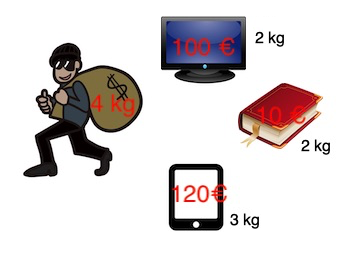
\includegraphics[scale=0.5]{Sac}
\end{center}
\begin{enumerate}

	\item En respectant le poids maximal, déterminer ("sur papier") le nombre de façons de remplir le sac (on pourra présenter les résultats dans un tableau).
	\begin{tcolorbox}[enhanced,attach boxed title to top center={yshift=-3mm,yshifttext=-1mm},
		colback=blue!5!white,colframe=blue!75!black,colbacktitle=blue!25!black,
		title=solution :, fonttitle=\bfseries,
		boxed title style={size=small,colframe=green!25!black} ]
	\begin{center}
		\begin{tabular}{ | m{2cm} | m{2cm} | m{2cm}| m{2cm} | m{2cm} |} 
			\hline
			Possibilités&n°1&n°2 & n°3 &n°4\\ 
			\hline
			Objets&A& B & C&A+B \\ 
			\hline
			Valeur (€)&100 & 10 & 120 &100+10=110\\ 
			\hline
			poids (kg)&2& 2 & 3 &2+2=4\\ 
			\hline
		\end{tabular}
	\end{center}
\end{tcolorbox}
	\hrule 
	\item Indiquer quel est le choix le plus profitable au voleur.
	\begin{tcolorbox}[enhanced,attach boxed title to top center={yshift=-3mm,yshifttext=-1mm},
		colback=blue!5!white,colframe=blue!75!black,colbacktitle=blue!25!black,
		title=solution :, fonttitle=\bfseries,
		boxed title style={size=small,colframe=green!25!black} ]
	Parmi les quatre possibilités, la n°3 est la plus profitable au voleur ( car 120€ > 110€ > 100€ > 10€).
\end{tcolorbox}
	
\end{enumerate}
\hrule
\hrule
\medskip
\exo Exercice débranché - $\star$  mais accès à la documentation officielle Python3\\
Soit la liste d'objets suivante où chaque objet est caractérisé par (un poids, une valeur) et un sac tel que $p_{max}=2,7$:\newline
L=[(0.2,300),(0.2,500),(0.1,250),(0.3,500),(1.3,2300),(0.8,2000),(1.3,2500)]
\vspace{2mm}
\begin{enumerate}
	\item Ecrire une liste triée par valeurs (décroissantes) puis une liste triée par rapports décroissants $\frac{\text{valeur}}{\text{poids}}$
		\begin{tcolorbox}[enhanced,attach boxed title to top center={yshift=-3mm,yshifttext=-1mm},
		colback=blue!5!white,colframe=blue!75!black,colbacktitle=blue!25!black,
		title=solution :, fonttitle=\bfseries,
		boxed title style={size=small,colframe=green!25!black} ]
	Attention le poids est donné avant la valeur ! \\
	valeurs (décroissantes):  [(1.3,2500),(1.3,2300),(0.8,2000),(0.2,500),(0.3,500),(0.2,300),(0.1,250)]\\
	$\frac{\text{valeur}}{\text{poids}}$:  [(0.8,2000),(0.2,500),(0.1,250),(1.3,2500),(1.3,2300),(0.3,500),(0.2,300)]\\
		En cas d'égalité, on peut placer les objets au hasard
		\end{tcolorbox}
	\vspace{2mm}
.
	
	\item Appliquer l'algorithme glouton sur ces deux listes et écrire une liste réponse uniquement constituée de 0 ou de 1. Commenter.
		\begin{tcolorbox}[enhanced,attach boxed title to top center={yshift=-3mm,yshifttext=-1mm},
		colback=blue!5!white,colframe=blue!75!black,colbacktitle=blue!25!black,
		title=solution :, fonttitle=\bfseries,
		boxed title style={size=small,colframe=green!25!black} ]
		Algorithme Sac appliqué à la liste 1:\tabto{0.2cm}$\rightarrow$  [\textcolor{red}{(1.3,2500),(1.3,2300)},(0.8,2000),(0.2,500),(0.3,500),(0.2,300),\textcolor{red}{(0.1,250)}]\\
		\tabto{0.2cm}$\rightarrow$ Reponse=[1,1,0,0,0,0,1] par rapport à la liste triée
		\tabto{0.2cm}$\rightarrow$ Reponse=[0,0,1,0,1,0,1] par rapport à la liste initiale
		\tabto{0.2cm}$\rightarrow$ Poids du Sac n°1: 2,7 \& Valeur du Sac n°1: 5050
		\tabto{0.2cm}$\rightarrow$ Le Sac n°1 est maximal ce qui ne signifie nécessairement que 5050 soit la solution optimale.
		\vspace{2mm}
		
			Algorithme Sac appliqué à la liste 2 :\tabto{0.2cm}$\rightarrow$   [\textcolor{red}{(0.8,2000),(0.2,500),(0.1,250),(1.3,2500)},(1.3,2300),\textcolor{red}{(0.3,500)},(0.2,300)]\\
		\tabto{0.2cm}$\rightarrow$ Reponse=[1,1,1,1,0,1,0] par rapport à la liste triée
		\tabto{0.2cm}$\rightarrow$ Reponse=[0,1,1,1,0,1,1] par rapport à la liste initiale
		\tabto{0.2cm}$\rightarrow$ Poids du Sac n°2: 2,7 \& Valeur du Sac n°2: 5750
		\tabto{0.2cm}$\rightarrow$ Le Sac n°2 est également maximal mais de valeur supérieur au Sac n°1 (ce qui ne prouve toujours rien sur son optimalité !). On peut néanmoins conclure que l'algorithme glouton donne une meilleure réponse avec le second critère.
		
	\end{tcolorbox}

		\item En Python, que renvoie les instructions \mintinline{python}{L.sort(key = lambda a : a[1])} et\\ \mintinline{python}{L.sort(key = lambda a : a[0], reverse=True)} ?
			
		\begin{tcolorbox}[enhanced,attach boxed title to top center={yshift=-3mm,yshifttext=-1mm},
			colback=blue!5!white,colframe=blue!75!black,colbacktitle=blue!25!black,
			title=solution :, fonttitle=\bfseries,
			boxed title style={size=small,colframe=green!25!black} ]
			https://docs.python.org/3/howto/sorting.html: \\ \textit{"list.sort() and sorted() have a key parameter to specify a function to be called on each list element prior to making comparisons."
				[...]accept a reverse parameter with a boolean value. This is used to flag descending sorts.}\newline
			
			Dès lors, on peut appeler une fonction \textbf{lambda} (nom donné à une fonction nommée "à la volée") pour trier des objets à un certain indice dans l'élément courant (si cet élément est une liste, un tuple,...)
			En conséquence, le tri sur \textbf{a[1]} signifie que l'on s'intéresse au deuxième élément du tuple, c'est à dire à la valeur dans cet exercice. Par ailleurs, \textbf{reverse=True} indique qu'il s'agit d'un tri "décroissant".\newline
			\tabto{0.2cm}$\rightarrow$  \textbf{L.sort(key = lambda a : a[1])}$\rightarrow$ Tri par valeur croissante: [(0.1, 250), (0.2, 300), (0.2, 500), (0.3, 500), (0.8, 2000), (1.3, 2300), (1.3, 2500)]\\
			\tabto{0.2cm}$\rightarrow$  \textbf{L.sort(key = lambda a : a[0], reverse=True)}$\rightarrow$ Tri par poids décroissant:[(1.3, 2300), (1.3, 2500), (0.8, 2000), (0.3, 500), (0.2, 300), (0.2, 500), (0.1, 250)]
			
			Dans le second tri, on pourra remarquer que Python place l'objet de valeur 2500 après celui de valeur 2300 .
		\end{tcolorbox}
\end{enumerate}	
\hrule
\medskip
\exo - exercice branché - $\star\star$  \\	
Il s'agit d'exécuter un algorithme "naïf" qui consiste à tester toutes les choix d'objets acceptables pour finir par choisir la meilleure. 
\begin{enumerate}
	\item Télécharger sur l'ENT le fichier \textbf{ex8.py}.
	\item Le code télechargé comporte plusieurs fonctions. La fonction \textbf{possibilites} de paramètre un entier $n$ permet d'afficher le nombre de choix possibles de $n$ objets (dans le sac du voleur).\\	Tester la fonction  \textbf{possibilites} pour   \(n \in \{3,4,5,6,7\} \). Conjecturer le nombre de façons de remplir le sac avec $n$ objets.
	\begin{tcolorbox}[enhanced,attach boxed title to top center={yshift=-3mm,yshifttext=-1mm},
		colback=blue!5!white,colframe=blue!75!black,colbacktitle=blue!25!black,
		title=solution :, fonttitle=\bfseries,
		boxed title style={size=small,colframe=green!25!black} ]
$2^3=8, 2^4=16,...2^7=128$ donc avec $n$ objets, on peut conjecturer que le nombre de façons de remplir le sac soit  $2^n$.
	\end{tcolorbox}
	
	\item La fonction \textbf{KPnaif} de paramètre une liste de couples  \textbf{(valeur en €, poids en kg)} et un entier $n$  retourne  un triplet constitué de la solution optimale obtenue par l'algorithme naïf pour le sac, la valeur du sac et le poids du sac. Tester l'algorithme et noter les durées d'exécution sur les 5 premiers jeux de données du fichier datas.txt, c'est à dire pour $n  \in \{4,7,8,10,15 \}$.
	
	\begin{tcolorbox}[enhanced,attach boxed title to top center={yshift=-3mm,yshifttext=-1mm},
		colback=blue!5!white,colframe=blue!75!black,colbacktitle=blue!25!black,
		title=solution :, fonttitle=\bfseries,
		boxed title style={size=small,colframe=green!25!black} ]
			n=4  \tabto{1.5cm}[(7,13),(4,12),(3,8),(3,10)] 30\\
		n=7 \tabto{1.5cm}[(442, 41),(525, 50),(511, 49),(593, 59),(546, 55),(564, 57),(617, 60)] 170\\
		n=8   \tabto{1.5cm}[(15, 2),(100, 20),(90, 20),(60, 30),(40, 40),(15, 30),(10, 60),(1, 1)] 102\\
		n=10  \tabto{1.5cm}[(92, 23),(57, 31),(49, 29),(68, 44),(60, 53),(43, 38),(67, 63),(84, 85),(87, 89),(72, 82)] 165\\
		n=15  \tabto{1.5cm}[(214, 113),(229, 118),(192, 98),(150, 80),(173, 90),(139, 73),(240, 120),(156, 82),(135, 70),(163, 87),(221, 115),\\
		\tabto{1.5cm}(201, 106),(149, 77),(184, 94),(210, 110)] 750\\
		
		
		
		%{\rowcolors{3}{gray!35!black!10}{green!70!yellow!40}
		\begin{tabular}{ |p{2.6cm}|p{1.3cm}|p{1.3cm}|p{1.3cm}|p{1.3cm}|p{1.3cm}| }
			\hline
			\multicolumn{6}{|c|}{KPnaif: Réponses et Durée d'exécution (en s) } \\
			\hline
			Objets&n=4&n=7&n=8& n=10&n=15\\
			\hline
			Durée   &1.291e-4& 2.129e-3&4.348e-3 & 2.100e-2 &1.137 \\
			Réponse   &\tiny([1,1,0,0], \newline11, 25)&\tiny ([0, 1, 0, 1, 0, 0, 1], \newline1735, 169)&\tiny([1, 1, 1, 1, 0, 1, 0, 0],\newline 280, 102) & \tiny([1, 1, 1, 1, 0, 1, 0, 0, 0, 0], \newline309, 165) &\tiny([0, 1, 1, 0, 1, 0, 1, 1, 1, 0, 0, 0, 1, 1, 0] ,\newline1458, 749) \\
			\hline
		\end{tabular}
		%}
		
		
		\vspace{2mm}
		* Calculs effectués sur 1000 itérations pour chaque fonction ; MacBook Pro IntelCore i5 2.4 GHz double coeur\\
		
	\end{tcolorbox}
	
	
	\item  A l'aide du logiciel de votre choix, représenter $t=f(n)$ où $t$ représente la durée d'exécution du programme.\\
	Donner une équation d'une courbe de tendance de la forme $t=a\times e^{b\times n}$ (donner les valeurs des paramètres a, b).
	\begin{tcolorbox}[enhanced,attach boxed title to top center={yshift=-3mm,yshifttext=-1mm},
		colback=blue!5!white,colframe=blue!75!black,colbacktitle=blue!25!black,
		title=solution :, fonttitle=\bfseries,
		boxed title style={size=small,colframe=green!25!black} ]
		\begin{center}
		Evolution exponentielle de la durée d'exécution de l'algorithme naïf\\
	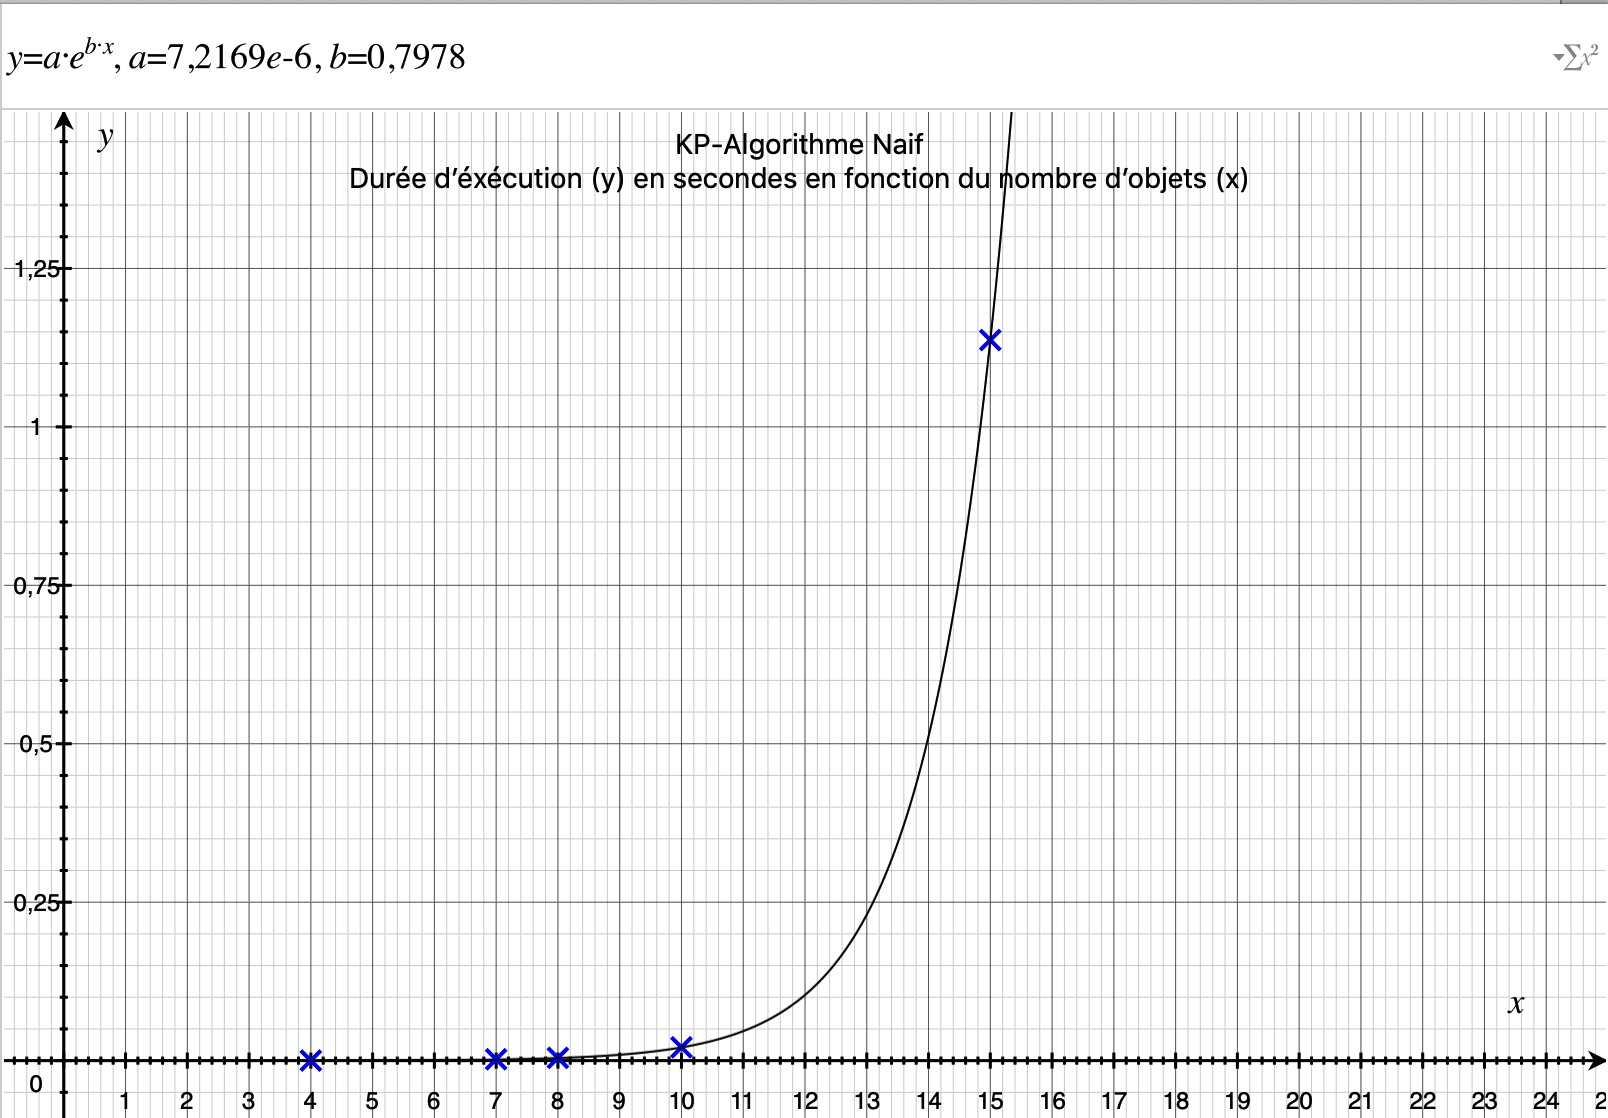
\includegraphics[width=90mm]{AlgoNaif}	
		\end{center}
	\end{tcolorbox}
	
	\item Quel est le temps d'exécution prédit par ce modèle lorsque n=50? Commenter le résultat obtenu.
	
\begin{tcolorbox}[enhanced,attach boxed title to top center={yshift=-3mm,yshifttext=-1mm},
	colback=blue!5!white,colframe=blue!75!black,colbacktitle=blue!25!black,
	title=solution :, fonttitle=\bfseries,
	boxed title style={size=small,colframe=green!25!black} ]
	
	On peut modéliser la durée d'exécution $t$ en fonction de $n$ par $t(n)=7,217\times 10^{-6} \times e^{0,7978\times n}$  où n est le nombre d'objets à voler. \\
	Ce modèle prédit, $t(50)=7,217\times 10^{-6} \times e^{0,7978\times 50} \approx 1521821054913  $s \\
	Il s'agit d'une durée proche de 50 000 ans !! Il n'est donc pas réaliste d'envisager une recherche de solution optimale par "force brute" même pour des ensembles relativement petits.	
		\end{tcolorbox}
\end{enumerate}	
\end{document}








